\documentclass[a4paper,12pt]{article}
\usepackage[UTF8]{ctex}
\usepackage{tocloft}
\usepackage{graphicx}
\usepackage{caption}
\usepackage{hyperref}
%定义图片位置
\graphicspath{{./Figure}}
%重定义图注
\captionsetup[figure]{name=Figure, labelsep=colon}
% 重定义目录命令,以居中显示目录标题
\renewcommand{\contentsname}{\hfill\bfseries\Large 目录\hfill}   
\renewcommand{\cftaftertoctitle}{\hfill}

%调整红框
\hypersetup{
    colorlinks=false,% 使用边框而不是颜色链接
    pdfborderstyle={/S/U/W 0} % 无边框
}

% 定义一个用于图表引用的命令,仅为引用添加红色边框
\newcommand{\figref}[1]{%
    \begingroup
    \hypersetup{pdfborderstyle={/S/S/W 1}, linkbordercolor={1 0 0}} % 方框样式,红色
    \ref{#1}%
    \endgroup
}

\begin{document}
% 更改封面的字体样式
\title{\huge My Test Document}
\author{{\large knight-zzm}}
\date{\today}
\maketitle
\thispagestyle{empty} % 封面页无页码
\newpage

\tableofcontents
\thispagestyle{empty} % 无页码
\newpage
\pagenumbering{arabic}
\section{练习latex 论文写作}
This is the introduction.

\subsection{图表的创建和引用}
    The above data is combined to form a correlation heat map bettween features,as show in Fig.\figref{fig:time-freq}
    \begin{figure}[h]
        \centering
        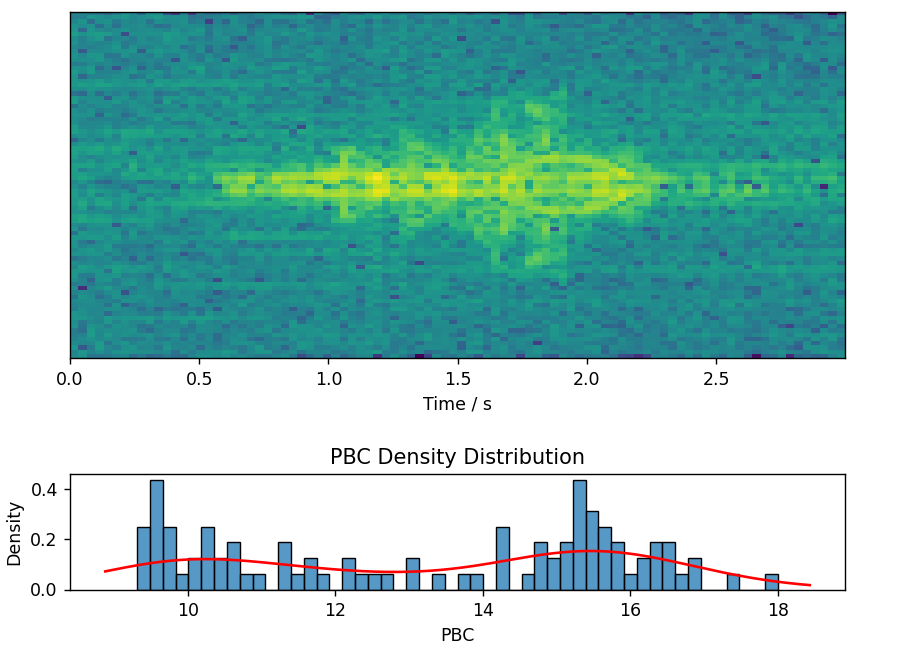
\includegraphics[width=1\textwidth]{时频图和PBC分布图.png}
        \caption{时频图和PBC分布图}
        \label{fig:time-freq}
    \end{figure}

\subsection{公式编辑和引用}
    1. 太阳高度角 \(\alpha_{s}\) [3] 
    %单独显示公式要加\[\]
    \[\sin \alpha_s=\cos \delta \cos \varphi \cos \omega+\sin \delta \sin \varphi\]
    太阳方位角 \(\gamma_{s}[4]\)
    \(\cos \gamma_{s}=\frac{\sin \delta-\sin \alpha_{s} \sin \varphi}{\cos \alpha_{s} \cos \varphi}\)
    其中 \(\varphi\) 为当地纬度, 北纬为正; \(\omega\) 为太阳时角
    \[\omega=\frac{\pi}{12}(S T-12)\]
    其中 \(D\) 为以春分作为第 0 天起算的天数, 例如, 若春分是 3 月 21 日, 则 4 月 1 日对应 \(D=11\) 。
    2. 法向直接辐射辐照度 DNI (单位: \(\mathrm{kW} / \mathrm{m}^{2}\) ) 是指地球上垂直于太阳光线的平面单位面积
    上、单位时间内接收到的太阳辐射能量, 可按以下公式近似计算[6]
    $$
	\begin{array}{l}
        {\mathrm{DNI}=G_{0}\left[a+b\exp\left(-\frac{c}{\sin\alpha_{e}}\right)\right],}\\ 
        {a=0.4.37-0.00821(6-H)^{2},}\\ {=0.505+0.0088667-H^{2},}\\ 
        {c=0.2711+0.01858(2.57-H)^{2},}\end{array}
	$$
        其中
        $G_{\mathrm{0}}$ 
        为太阳常数,其值取为1.366 kW/m?,H 为海拔高度(单位:km).
        3.定日镜场的输出热功率
        $E_{\mathrm{frield}}\ {\mathcal{N}}_{J}$ 
        $$
        E_{\mathrm{field}}=\mathrm{DN}\Lambda\sum_{i}^{N}A_{i}\eta_{i},
	$$
    其中 DNI 为法向直接辐射辐照度;N为定日镜总数(单位:面);A:为第i面定日镜采光
	面积(单位:m-\);
	$\eta_{i}$ 
	
	为第i面镜子的光学效率。
    

\subsection{表格编辑和引用}
    \begin{tabular}{|c|c|c|c|}
        \hline
        \multicolumn{2}{|c|}{MCM} & \multicolumn{2}{|c|}{ICM} \\
        \hline
        A & 连续型 & D & 运筹学/网络科学\\
        \hline
        B & 离散型 & E & 环境科学\\
        \hline
        C & 大数据 & F & 政策\\
        \hline
    \end{tabular}
    
    \begin{tabular}{rc}
    Apples & Green\\
    \hline 
    Strawberries & Red \\
    \cline{1-1}
    Oranges & Orange \\
    \end{tabular}
    
    \begin{tabular}{|r|l|}
    \hline
    8 & here's \\
    \cline{2-2}
    86 & stuff\\
    \hline \hline 
    2008 & now \\
    \hline 
    \end{tabular}

\end{document}

